\documentclass[10pt,twocolumn]{article}
\usepackage[margin=0.78in]{geometry}
\usepackage{graphicx,booktabs,longtable,array,amsmath,amssymb,natbib,microtype,placeins}
\usepackage[hidelinks]{hyperref}
\usepackage[font=small]{caption}
\setlength{\parindent}{0pt}\setlength{\parskip}{4pt}
\setlength{\columnsep}{0.24in}\sloppy
\newcommand{\evidencelabel}[1]{\textbf{#1}\enspace}
\title{Confirmatory evaluation separates uncertainty calibration from discovery performance in materials active learning}
\author{Renjie Li\\[2pt]\normalsize Southwest University}
\date{}
\begin{document}\maketitle
\begin{center}\small\textbf{Internal review build. Submission is blocked pending verified metadata.}\end{center}

\begin{abstract}
Predictive uncertainty supports two distinct operations in materials active learning: interpreting predictive intervals and directing acquisition. We developed a role-decomposed framework that evaluates calibration-only, acquisition-only, joint and exploration-matched interventions without conflating these functions. V6 confirmation covered four Matbench tasks, two study-defined splits, Random Forest and ExtraTrees surrogates, and 40 paired seeds in each of 16 environments. Complex global and candidate-specific mappings did not improve their registered calibration or top-tail discovery outcomes. Residual-ratio scaling favored pooled campaign calibration, but only 8 of 16 environments shared that direction. Stagewise matched beta partly recovered the discovery loss of the original global mapping, yet remained below RAW. Independent P1 confirmation used seeds 8200--8239 and a conditional-quantile gradient-boosting surrogate. Stagewise matched beta was favorable relative to fixed matched beta for top-1\% recall nAUC, but not relative to RAW; the other four P1 alternatives were unsupported. Under the quantile surrogate, residual-ratio scaling worsened campaign calibration when used only for interval evaluation and reduced discovery when used only for acquisition. Mapping utility was therefore role-, model-, baseline- and environment-dependent, rather than a transferable property of recalibration alone. The evidence is limited to offline finite pools, composition-only descriptors, four task snapshots, two bagged-tree surrogates and one quantile-gradient-boosting surrogate.
\end{abstract}

\section{Introduction}
Finite-budget materials screening is governed by acquisition decisions, not
predictive accuracy alone
\citep{lookman2019active,xue2016adaptive,kusne2020closedloop,rohr2020metrics,hase2021olympus}.
Recent materials benchmarks likewise show that regression quality, uncertainty
quality, and task-relevant discovery metrics need not rank models identically
\citep{varivoda2023uq,riebesell2025matbenchdiscovery}. In an active-learning
campaign, uncertainty informs both the interpretation of predictions and the
choice of the next candidate. Upper-confidence-bound (UCB) acquisition makes
the second role explicit by combining a predictive mean with an
uncertainty-weighted exploration term
\citep{auer2002ucb,srinivas2010gpucb,shahriari2016bo,frazier2018tutorial}.

These roles depend on different properties of the uncertainty signal.
Calibration concerns probabilistic interval behavior; uncertainty ranking
orders candidates; exploration pressure allocates a finite budget; and
trajectory feedback changes later training data. These properties interact,
but they are not interchangeable
\citep{gneiting2007proper,kuleshov2018calibrated,guo2017calibration,angelopoulos2023conformal,mandi2022decision,wilder2019decision,donti2017task}.
A global uncertainty multiplier may change interval widths and the effective
UCB coefficient without changing candidate order. A candidate-specific
mapping can also change the order, which can redirect later training data and
query trajectories.


Evidence across Bayesian optimization and materials active learning is mixed:
recalibration can improve optimization in some model--dataset combinations,
but calibration quality does not determine regret or OOD discovery utility on
its own \citep{foldager2023uncertainty,jiang2026calibration,dale2025ood}.
This motivates intervention-level separation of evaluation and acquisition
rather than treating calibration as a universal proxy for decision quality.

Most policy benchmarks compare these components jointly. A different query
trajectory can then reflect changed interval scale, changed candidate ranking,
changed effective exploration, trajectory feedback, or several pathways at
once. Such comparisons estimate policy performance but do not localize the
role through which a transformation acts.

We address this identification problem with an operationally role-decomposed
framework: calibration-only, acquisition-only, and joint mappings are compared
with identity and matched-exploration controls
(Fig.~\ref{fig:role-decomposition}). Fixed and stagewise matched-beta controls
isolate exploration pressure without treating it as probabilistic
recalibration. The framework is the contribution; it is neither a new
surrogate model nor a claim of a universally optimal acquisition algorithm.

Development evidence is necessary for strategy construction, but it cannot
serve as independent confirmation. We froze the environment set, strategies,
endpoints, seed blocks, and multiplicity families before confirmation. Four
Matbench regression tasks, two study-defined splits, and two tree ensembles
yielded 16 environments
\citep{dunn2020matbench,ward2018matminer,butler2018mlmaterials}.
Forty disjoint paired seed blocks then tested calibration error and discovery
performance separately.

The resulting confirmation asks which tested transformations change
calibration, acquisition, both, or neither. It retains unfavorable results,
prespecified environment heterogeneity, and descriptive comparisons without
promoting them to new confirmatory claims. Supplementary Table~S12 compares
this role separation and evidence boundary with representative prior work.

\begin{figure*}[tbp]
\centering
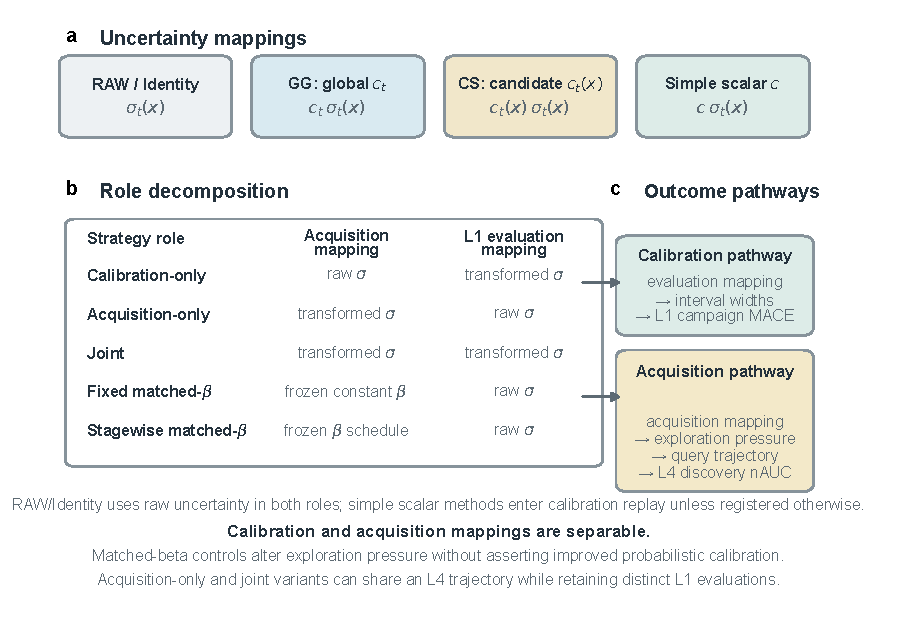
\includegraphics[width=.99\linewidth]{figures_v6/Figure1_uncertainty_role_decomposition.pdf}
\caption{Uncertainty mappings and role-decomposed evaluation. RAW or identity
uses unmodified uncertainty, GG applies a global mapping, CS applies a
candidate-specific mapping, and simple scalar methods apply one calibration
factor. Calibration-only, acquisition-only, and joint variants place the
transformed uncertainty in different campaign roles. The calibration pathway
changes interval widths and L1 campaign MACE. The acquisition pathway changes
exploration pressure, the query trajectory, and L4 discovery nAUC. Fixed and
stagewise matched-beta controls change exploration pressure while retaining
raw uncertainty for evaluation. The schematic contains no effect estimate.}
\label{fig:role-decomposition}
\end{figure*}

\section{Methods}

\subsection{Evidence classes, environments, and seed separation}
The V6 confirmation comprised four registered Matbench regression tasks
(\texttt{matbench\_expt\_gap}, \texttt{matbench\_mp\_gap},
\texttt{matbench\_log\_gvrh}, and \texttt{matbench\_log\_kvrh}), two split
types (IID-record and chemical-system-group out-of-distribution), and two
related tree-ensemble models (Random Forest and ExtraTrees). Their Cartesian
product yielded 16 task $\times$ split $\times$ model environments. The
environment set was frozen before confirmation and retained without
post-outcome selection.

Sentinel validation used seeds 6000--6009, and broad development used seeds
6100--6109. Independent confirmation used seeds 7000--7039. Confirmation
trajectories therefore did not enter strategy selection, matched-beta
construction, or policy tuning. Earlier V2, V3, and V5-RC1 stages supplied
exploratory, calibration-evaluation, development, selection, and historical
locked evidence. They document method provenance in Supplementary Fig.~S1 but
were not pooled with V6.

\subsection{Data roles and study-defined splits}
Each task snapshot was partitioned into mutually exclusive source, target, and
diagnostic roles. The source role supplied the seeded initial labelled set.
The target role was the finite candidate pool; a target label entered model
fitting only after that candidate had been queried. The diagnostic role was
never queried and never used to fit the surrogate or an uncertainty mapping;
its labels were read only by checkpoint evaluation. The split validator
required the three roles to be disjoint and exhaustive.

The IID-record split used a seeded permutation with approximately 20\% source,
60\% target, and 20\% diagnostic records. The chemical-system OOD split kept
all compositions with the same sorted element set in one role and assigned
whole groups toward the same proportions. No chemical system crossed roles.
These were study-defined splits over local Matbench task snapshots; the
original Matbench folds were not used.

\subsection{Descriptors and surrogate models}
Formula parsing used pymatgen 2024.10.29 \texttt{Composition}. Each task used
a deterministic, lexicographically ordered elemental atomic-fraction vector
plus total atom count and number of elements: 83 descriptors for experimental
gap and 86 for the other tasks. No feature scaling was applied to surrogate
fitting. The element vocabulary was constructed once over the complete task
without labels, a transductive preprocessing choice that exposes global
element presence but not target values. Random Forest used 80 bootstrap trees, squared-error splits,
unrestricted depth, minimum leaf size two, all features, and one worker
\citep{breiman2001rf,meinshausen2006qrf,wager2014confidence,mentch2016uncertainty}.
ExtraTrees used 80 bootstrap-bagged ExtraTree regressors with random split
thresholds and otherwise matched tree settings
\citep{geurts2006extratrees}. Tree means were averaged; population tree
dispersion was the uncertainty signal, floored at $10^{-8}$. These settings
were common to the compared strategies, so policy differences arose from the
registered uncertainty and acquisition mappings rather than a change of
surrogate class.

\subsection{Campaign geometry and endpoints}
For every task and split, the initial labeled count was
$\max(30,\mathrm{round}(0.01N))$ from the source role; batch size was
$\max(1,\mathrm{round}(0.01N))$; and maximum queries were
$\max(1,\mathrm{round}(0.20N_{\mathrm{target}}))$. Models were retrained after
each simultaneous batch. Ties used descending score and then ascending stable
record index; queried records were removed before rescoring. This deterministic
tie rule ensured that a policy and seed defined one reproducible query
trajectory.

L1 was campaign mean absolute coverage error (MACE), for which lower values
were better. Nominal coverages were 50\%, 80\%, 90\%, and 95\%. At the
initial, 25\%, 50\%, and 75\% campaign checkpoints, MACE was the mean of the
four absolute empirical-minus-nominal coverage errors on the diagnostic role;
the four checkpoint values received equal weight. Gaussian intervals used the
tree mean and effective standard deviation. L1 therefore evaluates the
calibration consequence of an uncertainty mapping along a campaign, rather
than the number of high-value materials found.

L4 was top-1\% recall normalized area under the curve (nAUC), for which higher
values were better. The target set comprised the highest
$\max(1,\lceil0.01N_{\mathrm{target}}\rceil)$ selectable targets, ordered by
target and then stable ID. Recall was integrated against queried-budget
fraction by the trapezoid rule, including the initial state at budget fraction
zero, and divided by the observed x-range. L4 depends on the ordered sequence
of queried candidates and therefore assesses a different consequence of the
policy from L1.

\subsection{Uncertainty transformation and acquisition decomposition}
Let $\mu_t(x)$ and $\sigma_t(x)$ denote the surrogate mean and raw uncertainty
for candidate $x$ at campaign step $t$. The registered raw UCB score was
\begin{equation}
a_{\mathrm{RAW}}(x,t)=\mu_t(x)+\beta\sigma_t(x).
\end{equation}
The Gaussian-global (GG) mapping used a fitted global factor $c_t$,
\begin{equation}
a_{\mathrm{GG}}(x,t)=\mu_t(x)+\beta c_t\sigma_t(x),
\end{equation}
with
\begin{equation}
\resizebox{.96\columnwidth}{!}{$\displaystyle c_t=\max\!\left(10^{-8},
\frac{\operatorname{median}_{i\in\mathcal O_t}
|y_i-\hat\mu_{i,\mathrm{OOB}}|/
\max(\hat\sigma_{i,\mathrm{OOB}},10^{-8})}
{0.67448975}\right).$}
\end{equation}
Here $\mathcal O_t$ contains currently labelled records with at least eight
finite OOB predictions. The mapping was refitted after every campaign update;
insufficient OOB support returned identity scaling. Frozen V5-derived GG and
CS policies retain their historical ordered queried-target/OOB pairing for
trajectory identity. New scalar mappings use aligned training-order OOB
targets.

The candidate-specific (CS) mapping used $c_t(x)$,
\begin{equation}
a_{\mathrm{CS}}(x,t)=\mu_t(x)+\beta c_t(x)\sigma_t(x).
\end{equation}
Thus, GG changes the uncertainty scale at a campaign step, while CS can also
change the relative uncertainty contribution across candidates. The selected
CS model uses standardized log raw uncertainty with an intercept. It samples
at most 20,000 unequal-target OOB pairs and minimizes a top-10\%-weighted
pairwise logistic ranking loss plus $0.01$ coefficient and mean-log-scale
penalties. Candidate log scales are clipped to
$[\log(0.25),\log(4)]$; fewer than 30 labelled records or insufficient OOB
support returns the raw policy. The historical CS comparator uses six local
features (raw uncertainty, leaf density, descriptor distance, predictive-mean
percentile, local standardized residual, and local residual dispersion).

For the NLL scalar, aligned OOB residuals $r_i$ determine
\begin{equation}
\resizebox{.96\columnwidth}{!}{$\displaystyle \hat c_{\mathrm{NLL}}=\arg\min_{0.05\le c\le20}
\frac{1}{|\mathcal O_t|}\sum_{i\in\mathcal O_t}
\left[\log(c\sigma_i)+\frac{r_i^2}{2c^2\sigma_i^2}\right]
=\operatorname{clip}_{[0.05,20]}
\sqrt{\operatorname{mean}(r_i/\sigma_i)^2}.$}
\end{equation}
The residual-ratio scalar instead uses
$\hat c_{\mathrm{RR}}=\operatorname{clip}_{[0.05,20]}
\{\operatorname{median}(|r_i|/\sigma_i)/0.6744897501960817\}$.
Both use OOB, not held-out diagnostic, residuals; both are refitted each round
and affect calibration evaluation only in their registered comparisons.

The two matched-beta controls retained raw $\sigma_t(x)$ and changed only the
exploration coefficient:
\begin{align}
a_{\mathrm{fixed}}(x,t) &=
\mu_t(x)+\beta_{\mathrm{fixed}}\sigma_t(x),\\
a_{\mathrm{stage}}(x,t) &=
\mu_t(x)+\beta_{s(t)}\sigma_t(x).
\end{align}
For each held-out task, $\beta_{\mathrm{fixed}}$ was the median across
environment-level medians of Original-GG effective beta from the other three
tasks and development seeds 6100--6109. The same leave-one-task-out rule was
applied separately within budget stages $[0,0.25)$, $[0.25,0.50)$,
$[0.50,0.75)$, and $[0.75,1]$ to obtain $\beta_{s(t)}$. The resulting
task-specific constant and schedule were frozen before confirmation; no stage
required fallback. Confirmation outcomes did not enter either value. The
controls consequently test changes in exploration pressure without asserting
that raw probabilistic uncertainty was recalibrated.

The calibration and acquisition roles were assigned independently
(Fig.~\ref{fig:role-decomposition}). Calibration-only strategies acquired with raw
$\sigma$ and evaluated L1 with transformed $\sigma$. Acquisition-only
strategies acquired with transformed $\sigma$ and evaluated L1 with raw
$\sigma$. Joint strategies used transformed $\sigma$ for both operations.
Matched-beta controls acquired with the frozen beta policy and evaluated with
raw $\sigma$. Identity used raw $\sigma$ in both roles. Simple scalar methods
entered calibration replay unless a different role was explicitly registered.

Acquisition-only and joint variants can have identical L4 results because L4
is a functional of the acquisition trajectory. When two variants use the same
acquisition mapping, stable tie rules yield the same ordered queries even if
their L1 evaluation mappings differ. They remain distinct strategies for L1,
where the reported interval widths depend on whether raw or transformed
uncertainty is evaluated.

\subsection{One complete campaign step}
At each step the implementation executed the following fixed sequence:
\begin{enumerate}
\item fit the registered surrogate to all currently labelled source and queried
target records using the deterministic round-specific seed;
\item compute candidate and diagnostic predictive means and raw ensemble
standard deviations;
\item fit the registered mapping from eligible labelled OOB records, or retrieve
the frozen fixed/stagewise beta;
\item construct the registered UCB score and order candidates by descending
score, breaking ties by ascending stable record ID;
\item query the leading batch, reveal only those target labels, and append them
to the labelled set;
\item refit at registered checkpoints, apply the evaluation mapping to the
untouched diagnostic role, and record calibration quantities;
\item update recall against the fixed top-target set and, after the campaign,
compute the registered calibration and discovery endpoints.
\end{enumerate}




\subsection{Strategies and registered comparisons}
The frozen design compared GG and CS calibration-only variants with RAW on L1.
It compared their acquisition-only and joint policies with RAW on L4. Fixed
and stagewise matched-beta controls were compared with Original GG on L4. NLL
and residual-ratio scalar scaling were compared with Identity Control on L1.
Residual-ratio scaling versus the development-selected CS joint policy was
estimation-only, and the cross-endpoint direction table was descriptive.

Original GG denotes the joint GG policy with nominal $\beta=1$, whereas
development-selected GG denotes the historically selected policy with nominal
$\beta=0.5$. Machine identifiers remain unchanged and are mapped to display
names in \path{tables/display_name_mapping.csv}. Acquisition-only and joint
variants can share L4 values because L4 depends on their common acquisition
trajectory. They remain distinct for L1 when their evaluation mappings differ.

\subsection{Locked inference and result control}
Every effect was defined as strategy minus baseline. The pooled inferential
unit was the registered seed block: within each of the 40 shared seeds, the
effect was averaged equally across all 16 environments, and inference was
performed on those 40 paired block effects. The 640 environment-seed
observations were not treated as independent scientific replicates.
Confidence intervals used 10,000 paired bootstrap samples, and confirmatory
p-values used 10,000 paired sign-flip permutations with add-one p-values.
Benjamini--Hochberg correction was applied separately within the four frozen
families. A 40-pair completeness gate was required for every registered
environment; all 176 gates passed.

Task-, split-, model-, and environment-level estimates were retained as
heterogeneity diagnostics and did not replace pooled inference. They were
reported to reveal transportability across the locked environment set, not to
select a favorable subgroup. H6 and H7 were descriptive only. Analysis inputs
were frozen before confirmation outcomes, and the result tables were bound by
\path{locks/v6_p0_confirmation_inference_result_lock.json}. No new
contrast, environment selection, statistical test, or model run was
introduced for this revision.

This statement applies to the locked V6 analysis. A separately prespecified
P1 extension was frozen after V6 and before any P1 outcome. It uses disjoint
sentinel (8000--8004), development (8100--8109), and confirmation
(8200--8239) seeds, and its multiplicity families cannot be pooled with V6.

\subsection{Prespecified P1 extension}
The P1 extension adds a non-bagged conditional-quantile mechanism. A central
gradient-boosting regressor estimates $\mu(x)$, while regressors at quantiles
0.16 and 0.84 estimate $q_{.16}(x)$ and $q_{.84}(x)$. The registered spread is
\begin{equation}
 \sigma_q(x)=\max\left\{\frac{q_{.84}(x)-q_{.16}(x)}
 {2\Phi^{-1}(.84)},10^{-8}\right\}.
\end{equation}
It is an interval-derived conditional predictive-spread proxy, not a
decomposition into epistemic and aleatoric uncertainty. Three role arms share
the same surrogate hyperparameters: raw mapping, residual-ratio
calibration-only, and residual-ratio acquisition-only. Five-fold cross-fitted
labelled residuals fit the scalar; diagnostic targets never fit a mapping.

The P1 endpoint registry adds coverage, width, interval score, Gaussian NLL,
Gaussian-proxy CRPS, standardized-residual and conditional-coverage
diagnostics, along with top-5\%/10\% recall, regret, enrichment, time-to-hit,
random-gain, and budget-segment summaries. Only the prospectively designated
L1 and L4 contrasts are confirmatory. The compute gate required complete environment pairs. A compute-only amendment, timestamped 2026-08-01T18:30:00+08:00 before any confirmation outcome, changed only scheduling and resource limits. The completed run comprised 3,520 jobs between 2026-08-01T11:45:33.733115Z and 2026-08-01T20:51:14.238681Z (9.095 h elapsed), with no failed jobs; peak memory, CPU time and peak temporary storage were not instrumented and are therefore not estimated.

\subsection{Reproducibility and audit trail}
The frozen strategy map records the acquisition and L1 evaluation mapping for
each policy. The endpoint registry fixes direction and aggregation, while the
contrast table fixes the strategy, baseline, and multiplicity family. The
pair-completeness table confirms that all required environments contain the
same 40 confirmation seeds. The inference lock binds pooled effects,
confidence intervals, p-values, and adjusted decisions.

Figures read stored rows directly, and rounding is confined to printed
labels. Supplementary Information provides the full registered results,
environment diagnostics, completeness gates, strategy registry, coefficient
tables, evidence lineage, and source hashes. No historical effect contributes
to a V6 estimate, interval, or p-value.

\section{Results}
\subsection{Locked analysis and reporting conventions}
L1 was lower-is-better campaign MACE, and L4 was higher-is-better top-1\%
recall nAUC. Every effect was strategy minus baseline. Pooled inference used
40 paired seed blocks, each averaging the 16 environments equally.
Confidence intervals used the registered paired bootstrap, and p-values used
the registered paired sign-flip procedure. Benjamini--Hochberg correction was
applied within each frozen family. Environment estimates remained
heterogeneity diagnostics.

\subsection{Complex calibration scaling did not improve calibration error}
GG calibration-only scaling increased L1 relative to RAW (effect, 0.065777;
95\% CI, 0.062782 to 0.068971; adjusted $p=1.000$). The effect was unfavorable
in all 16 environments. CS calibration-only scaling was also unfavorable at
the pooled level (effect, 0.095898; 95\% CI, 0.090827 to 0.100888; adjusted
$p=1.000$), with heterogeneous environment estimates. Values near one reflect
effects opposite to the registered lower-is-better alternative. They do not
show equivalence or absence of an effect.

\begin{figure*}[tbp]
\centering
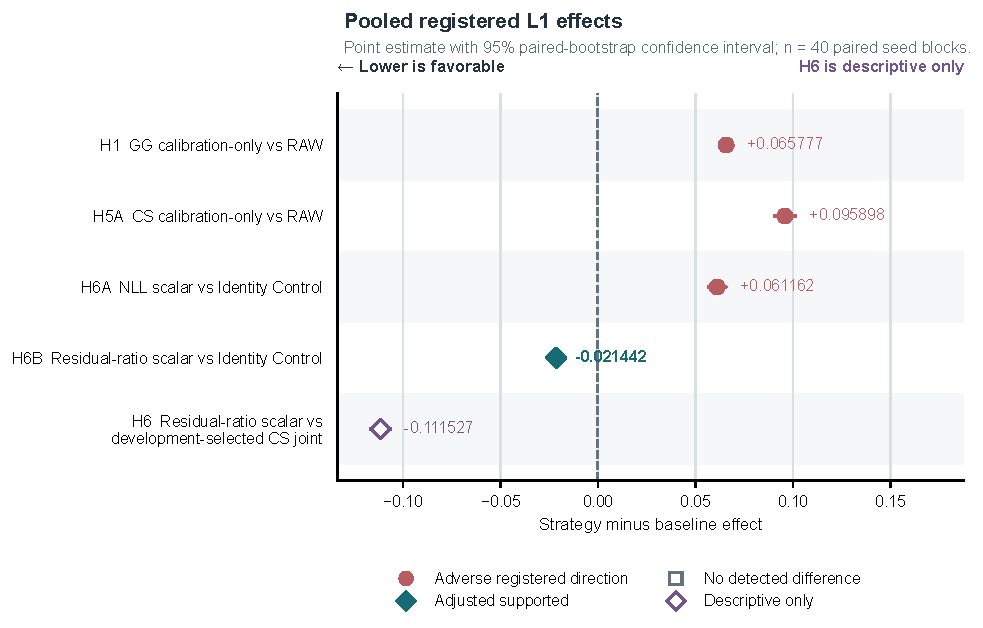
\includegraphics[width=.99\linewidth]{figures_v6/Figure2_L1_pooled_effects.pdf}
\caption{Pooled registered L1 effects. Effects are strategy minus baseline,
and lower values favor the strategy. Points and horizontal lines are locked
pooled effects and 95\% paired-bootstrap confidence intervals. Residual-ratio
scaling versus development-selected CS is descriptive only and has no binary
test. Residual-ratio scaling versus Identity Control remained supported after
family-specific correction, but only 8 of 16 environment estimates shared the
pooled favorable direction.}
\label{fig:l1-pooled}
\end{figure*}

\subsection{Complex acquisition and joint scaling did not improve discovery}
GG acquisition-only scaling reduced L4 relative to RAW (effect, -0.076313;
95\% CI, -0.085283 to -0.067686; adjusted $p=1.000$). GG joint, nominal
$\beta=1$, had the same point estimate and a separately resampled 95\% CI of
-0.085393 to -0.067613 (adjusted $p=1.000$). CS acquisition-only scaling and
the development-selected CS joint policy were also unfavorable (both effects,
-0.034084; adjusted $p=1.000$). Their respective 95\% CIs were -0.039446 to
-0.028599 and -0.039606 to -0.028612. Neither complex mapping improved the
registered discovery outcome.

\subsection{Matched-beta controls distinguished fixed and stagewise exploration policies}
Fixed matched-beta showed no detectable L4 difference from Original GG
(effect, -0.000236; 95\% CI, -0.005992 to 0.005446; adjusted $p=0.936$).
This was not an equivalence test and does not establish identity or
interchangeability. Stagewise matched-beta increased L4 relative to Original
GG (effect, 0.031619; 95\% CI, 0.025535 to 0.037613; adjusted $p<0.001$).
All 16 environment estimates were favorable. The comparison identifies a
performance difference, not a unique causal mechanism.

Absolute pooled levels provide the necessary baseline: RAW was 0.641635,
Original GG was 0.565322, and stagewise matched-beta was 0.596941. Thus the
registered stagewise-minus-Original-GG effect was $+0.031619$, while the
stagewise-minus-RAW difference was $-0.044694$. The latter comparison is
descriptive, was not registered for a confirmatory p-value, and was not added
to a multiplicity family. Stagewise matched-beta therefore partly recovered
the discovery loss of Original GG but did not establish superiority or
noninferiority to RAW. Original GG is the H4 baseline because the earliest
registry named its alias, GG joint; the matched-beta control was designed to
isolate Original GG's effective exploration pressure, not to test overall
performance against RAW.

\begin{figure*}[tbp]
\centering
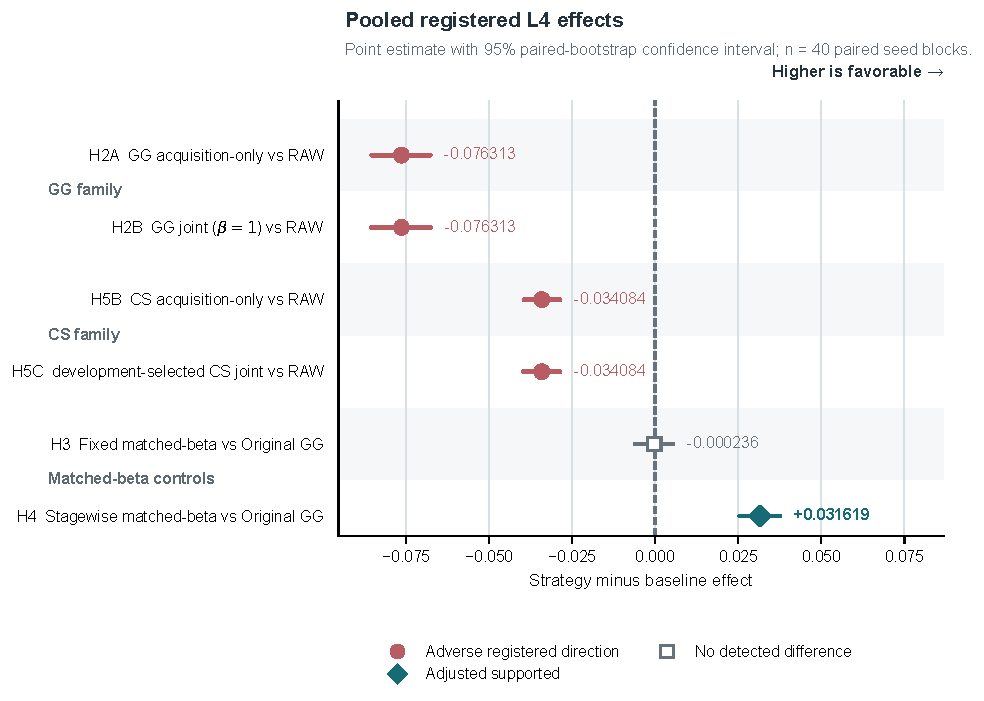
\includegraphics[width=.99\linewidth]{figures_v6/Figure3_L4_pooled_effects.pdf}
\caption{Pooled registered L4 effects. Effects are strategy minus baseline,
and higher values favor the strategy. Points and horizontal lines are locked
pooled effects and 95\% paired-bootstrap confidence intervals. Fixed
matched-beta showed no detectable difference and was not an equivalence test.
Stagewise matched-beta was the adjusted favorable registered comparison against Original GG. Acquisition-only
and joint GG or CS pairs share point estimates because each pair generated the
same acquisition trajectory.}
\label{fig:l4-pooled}
\end{figure*}

\subsection{Simple scalar scaling showed method-specific and heterogeneous calibration effects}
NLL scalar scaling increased L1 relative to Identity Control (effect,
0.061162; 95\% CI, 0.056963 to 0.065341; adjusted $p=1.000$).
Residual-ratio scalar scaling reduced pooled L1 (effect, -0.021442; 95\% CI,
-0.023667 to -0.019147; adjusted $p<0.001$). Only 8 of 16 environment
estimates shared the favorable direction, with effects ranging from -0.064399
to 0.019515. The pooled improvement therefore did not establish uniform
transportability. The corresponding absolute pooled levels were 0.069511 for
Identity Control and 0.048069 for residual-ratio scaling.

Residual-ratio scaling also had lower L1 than the development-selected CS
joint policy (effect, -0.111527; 95\% CI, -0.116235 to -0.106876). All 16
environment estimates were negative. This comparison was descriptive only and
had no binary test or multiplicity assignment. It does not establish
superiority or noninferiority.

\subsection{Environment heterogeneity and completeness}
Environment diagnostics qualified the pooled results without replacing them.
Stagewise matched-beta was favorable in 16 of 16 environments. The pooled
residual-ratio improvement was favorable in 8 of 16 environments. All
registered comparisons satisfied the 40-pair completeness requirement.

\begin{figure*}[tbp]
\centering
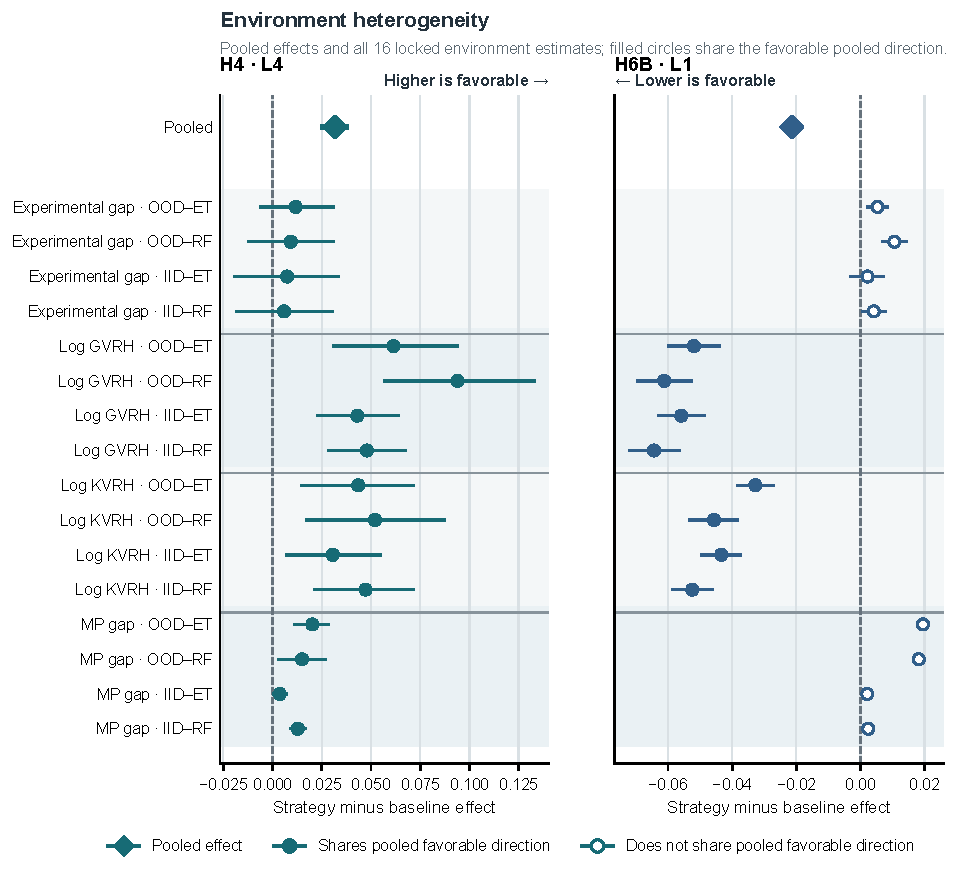
\includegraphics[width=.99\linewidth]{figures_v6/Figure4_H4_H6B_environment_heterogeneity.pdf}
\caption{Environment heterogeneity for stagewise matched-beta and
residual-ratio scaling. Points and horizontal lines are locked environment
effects and 95\% paired-bootstrap intervals, grouped by task. Stagewise
matched-beta was favorable in 16 of 16 environments, whereas residual-ratio
scaling was favorable in 8 of 16. These diagnostics qualify but do not replace
pooled inference.}
\label{fig:heterogeneity}
\end{figure*}

\subsection{Complete registered-result summary}
Table~\ref{tab:registered-summary} reports every registered pooled comparison.
The full-precision table, multiplicity families, and H7 descriptive direction
table are provided in Supplementary Information.

\FloatBarrier
\begin{table*}[!tbp]
\centering
\caption{Condensed V6 registered-result summary. Effects are strategy minus
baseline. L1 is lower-is-better and L4 is higher-is-better. The p-value column
reports the registered BH-adjusted result.}
\label{tab:registered-summary}
\scriptsize
\begin{tabular}{llrrrrl}
\toprule
ID & Endpoint & Effect & CI low & CI high & Adjusted $p$ & Interpretation\\
\midrule
H1  & L1 &  0.065777 &  0.062782 &  0.068971 & 1.000 & Unfavorable\\
H5A & L1 &  0.095898 &  0.090827 &  0.100888 & 1.000 & Unfavorable, heterogeneous\\
H2A & L4 & -0.076313 & -0.085283 & -0.067686 & 1.000 & Unfavorable\\
H2B & L4 & -0.076313 & -0.085393 & -0.067613 & 1.000 & Unfavorable\\
H5B & L4 & -0.034084 & -0.039446 & -0.028599 & 1.000 & Unfavorable, 16/16\\
H5C & L4 & -0.034084 & -0.039606 & -0.028612 & 1.000 & Unfavorable, 16/16\\
H3  & L4 & -0.000236 & -0.005992 &  0.005446 & 0.936 & No detectable difference\\
H4  & L4 &  0.031619 &  0.025535 &  0.037613 & $<0.001$ & Supported, 16/16\\
H6A & L1 &  0.061162 &  0.056963 &  0.065341 & 1.000 & Unfavorable\\
H6B & L1 & -0.021442 & -0.023667 & -0.019147 & $<0.001$ & Supported, heterogeneous\\
H6  & L1 & -0.111527 & -0.116235 & -0.106876 & -- & Descriptive only\\
\bottomrule
\end{tabular}
\begin{minipage}{.98\linewidth}\footnotesize\smallskip
One-sided BH-adjusted p-value refers to registered favorable-direction tests;
H3 and H4 retain their registered two-sided matched-beta tests. Tests targeted
the prospectively registered favorable direction. Effects lying in the
opposite direction therefore yield one-sided p-values near 1; such values do
not indicate equivalence or absence of an effect. H6 had no binary test or
multiplicity assignment.
\end{minipage}
\end{table*}



\subsection{Independent confirmation of exploration controls}
The P1 tree analysis distinguished performance against RAW from performance against a fixed exploration control. Stagewise matched beta was unfavorable relative to RAW for L4 (effect -0.040800, 95\% CI [-0.047582, -0.033996], raw $p=1.0000$, BH-adjusted $p=1.0000$). Its absolute mean L4 was 0.603956, compared with 0.644756 for RAW. Thus, time-varying exploration did not exceed the raw-uncertainty policy.

The same stagewise policy was favorable relative to fixed matched beta (effect 0.030320, 95\% CI [0.024001, 0.036682], raw $p=9.999\times10^{-5}$, BH-adjusted $p=0.00029997$). Absolute mean L4 was 0.573636 for fixed matched beta. This result supports a schedule-specific contrast against a mechanistic control, not overall superiority. Development-selected constant beta was also unfavorable relative to RAW (effect -0.017442, 95\% CI [-0.020936, -0.013972], BH-adjusted $p=1.0000$). Its absolute mean L4 was 0.627314.


\begin{table*}[!tbp]
\centering\scriptsize
\caption{Independent P1 registered comparisons. Effects are strategy minus baseline. L1 is campaign mean absolute coverage error, for which less is favorable; L4 is top-1\% recall nAUC, for which greater is favorable. Confidence intervals use 10,000 paired bootstrap resamples. BH adjustment was applied within the two prespecified P1 families.}
\label{tab:p1-primary}
\resizebox{\textwidth}{!}{%
\begin{tabular}{lllllllll}
\toprule
ID & Strategy & Baseline & Endpoint & Registered alternative & Effect & 95\% CI & BH-adjusted $p$ & Evidence-constrained interpretation\\
\midrule
P1\_C1 & Stagewise matched beta & RAW & L4 & greater & -0.040800 & [-0.047582, -0.033996] & 1.0000 & Opposed greater alternative\\
P1\_C2 & Stagewise matched beta & Fixed matched beta & L4 & greater & 0.030320 & [0.024001, 0.036682] & 0.00029997 & Supported in this comparison\\
P1\_C3 & Selected constant beta & RAW & L4 & greater & -0.017442 & [-0.020936, -0.013972] & 1.0000 & Opposed greater alternative\\
P1\_C4 & RR calibration-only & QGB RAW & L1 & less & 0.097439 & [0.095013, 0.099841] & 1.0000 & Opposed less alternative\\
P1\_C5 & RR acquisition-only & QGB RAW & L4 & greater & -0.009354 & [-0.014256, -0.004685] & 1.0000 & Opposed greater alternative\\
\bottomrule
\end{tabular}}
\begin{minipage}{.98\linewidth}\footnotesize\smallskip
P1\_C2 supports only the stagewise-versus-fixed matched-beta comparison. Effects opposite to a registered one-sided alternative yield adjusted $p$ values near 1; they do not establish equivalence or absence of an effect. Full machine identifiers and raw $p$ values are given in Supplementary Table~S14.
\end{minipage}
\end{table*}


\begin{figure*}[tbp]
\centering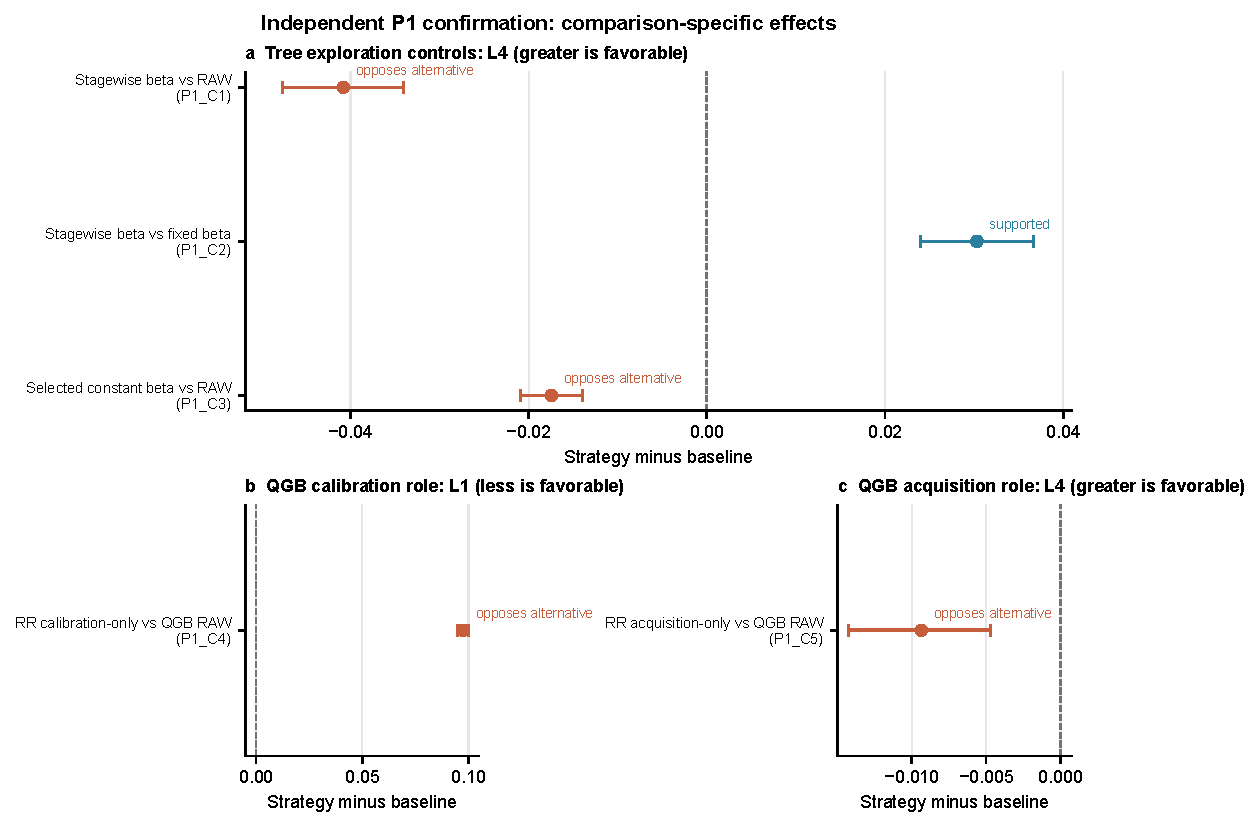
\includegraphics[width=.96\linewidth]{figures_p1_confirmation/P1_Figure01_registered_effects.pdf}
\caption{Independent P1 effects, grouped by endpoint and scientific role. Points are equal-environment paired seed-block means; bars are 95\% paired-bootstrap intervals. Panel a reports tree L4 contrasts, for which greater is favorable. Panel b reports the QGB calibration-only L1 contrast, for which less is favorable. Panel c reports the QGB acquisition-only L4 contrast, for which greater is favorable. P1\_C2 supports only stagewise matched beta relative to fixed matched beta. Orange effects oppose their registered alternatives. The inferential unit is one of 40 confirmation seed blocks, with family-specific BH adjustment.}
\label{fig:p1-effects}
\end{figure*}

\subsection{Role-specific residual-ratio scaling under the quantile surrogate}
The quantile-gradient-boosting (QGB) model provided a conditional predictive-spread proxy rather than a strict epistemic-uncertainty estimate. Residual-ratio calibration-only scaling preserved the QGB RAW acquisition path but increased L1 by 0.097439 (95\% CI [0.095013, 0.099841], BH-adjusted $p=1.0000$). Because lower L1 was registered as favorable, this positive effect represents worse campaign calibration. Absolute mean L1 increased from 0.090532 for QGB RAW to 0.187971.

Residual-ratio acquisition-only scaling preserved raw interval evaluation but reduced L4 by 0.009354 relative to QGB RAW (strategy-minus-baseline effect -0.009354, 95\% CI [-0.014256, -0.004685], BH-adjusted $p=1.0000$). Absolute mean L4 decreased from 0.622936 to 0.613582. The same fitted-scalar family was therefore unfavorable in both registered roles, but the endpoints and effect scales were distinct.

\subsection{Diagnostics, heterogeneity and robustness}
Task-level estimates showed that the favorable direction occurred in 2/4 tasks for stagewise beta versus RAW and 3/4 tasks for stagewise versus fixed beta. It occurred in 0/4, 0/4 and 0/4 tasks for the other registered comparisons. The IID and chemical-system OOD summaries retained the pooled direction for every contrast, but task effects varied markedly, especially for the two stagewise comparisons.

At the final QGB checkpoint, calibration-only scaling narrowed the mean 90\% interval while increasing MACE and the interval score relative to QGB RAW. Gaussian-proxy proper scores contained extreme tail values, so they are presented as descriptive diagnostics rather than used to rescue or overturn the registered L1 result. Fitted residual-ratio scalars varied across campaigns and stages, and quantile crossings were retained rather than filtered. Discovery trajectories confirmed that calibration-only and QGB RAW shared an acquisition path, whereas acquisition-only scaling reduced top-tail recall.

Leave-one-task-out estimates preserved the pooled effect direction for all five comparisons. Exploratory random-effects prediction intervals crossed zero for P1\_C1--P1\_C4 but not P1\_C5 (P1\_C5 interval [-0.012774, -0.005180]). These task, split, environment, proper-score, trajectory, crossing and scalar analyses are descriptive or exploratory; they do not form additional confirmatory families.

\begin{figure*}[tbp]
\centering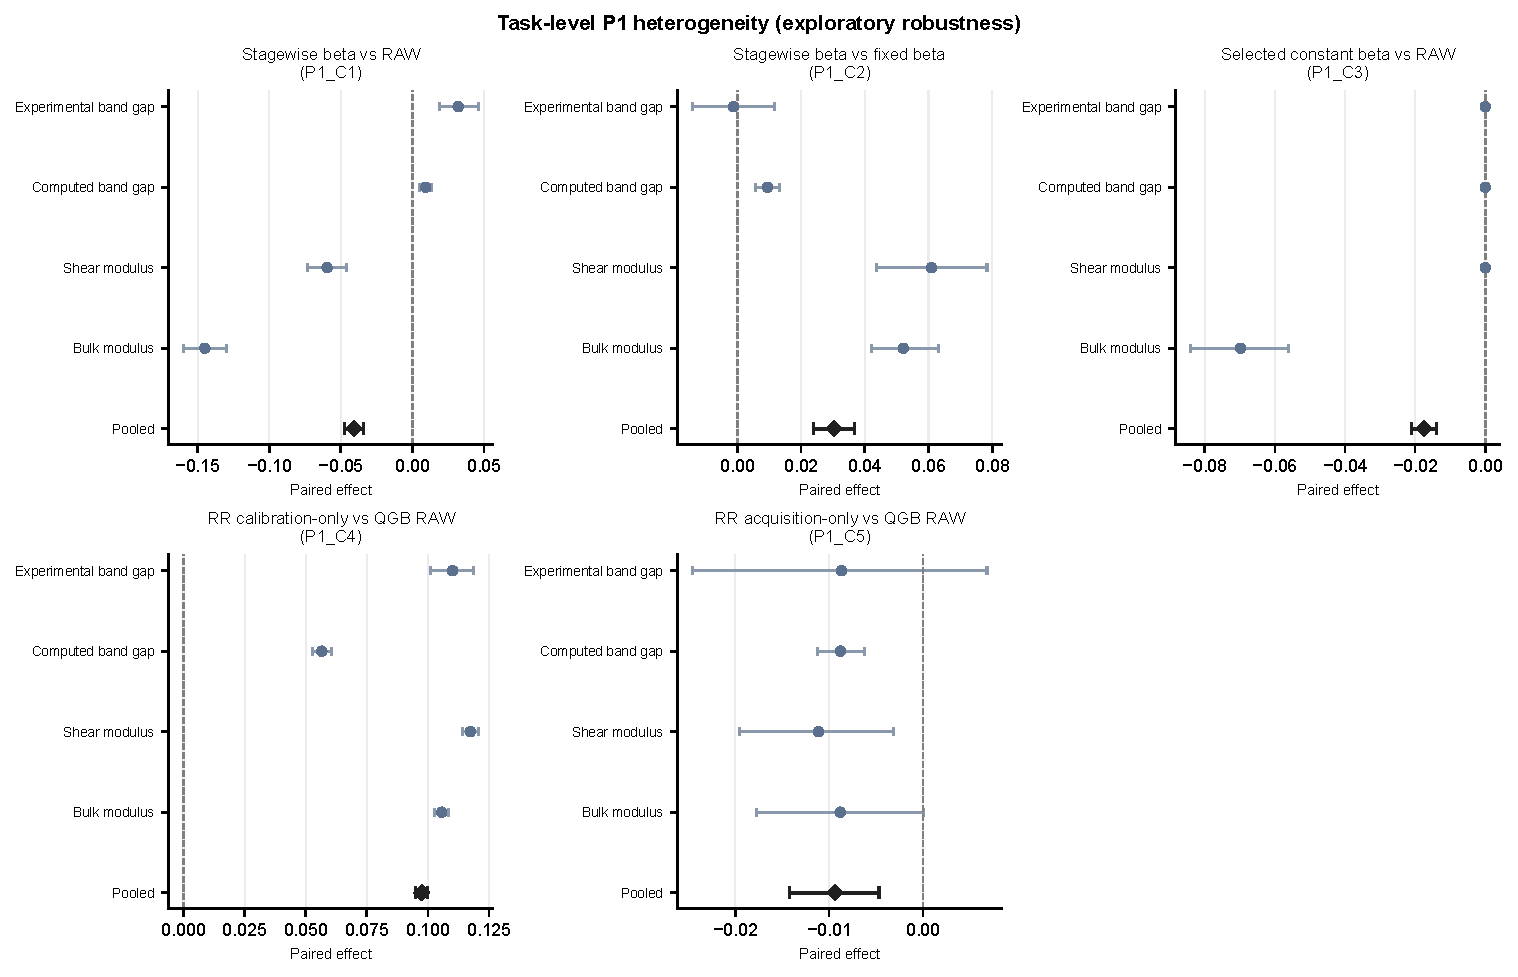
\includegraphics[width=.98\linewidth]{figures_p1_confirmation/P1_Figure02_environment_heterogeneity.pdf}
\caption{Task-level P1 heterogeneity. Circles and thin bars are task-specific exploratory estimates and 95\% paired-bootstrap intervals across 40 confirmation seeds. Diamonds and thick bars show the registered pooled effects. The four rows are scientific tasks; split/model repetitions are not treated as additional tasks. Full task $\times$ split $\times$ model environment estimates are descriptive and appear in Supplementary Figs.~S20--S22.}
\label{fig:p1-heterogeneity}
\end{figure*}
\begin{table*}[!tbp]
\centering
\caption{Claim-evidence classification for locked V6 and P1 results.}
\label{tab:claim-classification}
\small
\begin{tabular}{p{.17\linewidth}p{.23\linewidth}p{.52\linewidth}}
\toprule
Evidence class & Objects & Evidence-constrained conclusion\\
\midrule
V6 adjusted confirmation & H4, H6B & Supported registered comparisons; H4 is relative to Original GG and H6B is heterogeneous\\
V6 contradicted direction & H1, H2A, H2B, H5A--H5C, H6A & Prespecified favorable directions were not supported\\
V6 bounded null/descriptive & H3, H6, H7 & H3 found no detectable difference without testing equivalence; H6/H7 are descriptive\\
P1 supported comparison & P1\_C2 & Stagewise matched beta was favorable relative to fixed matched beta for L4 only\\
P1 unfavorable direction & P1\_C1, C3, C4, C5 & Effects opposed their registered favorable alternatives; this is not evidence of no effect\\
P1 exploratory robustness & Task, split, leave-one-task-out, random effects, Wilcoxon & Sensitivity and heterogeneity context only; no new confirmatory family\\
P1 descriptive diagnostics & Coverage, proper scores, trajectories, crossings, scalar distribution & Absolute-scale and pathway context only; no causal claim\\
\bottomrule
\end{tabular}
\end{table*}

\FloatBarrier

\section{Discussion}
\subsection{Calibration and discovery require separate intervention roles}
Calibration-only, acquisition-only and joint variants separate where an uncertainty mapping enters an active-learning campaign. L1 measures interval behavior along the campaign, whereas L4 measures top-tail discovery along the query trajectory. A mapping can therefore change one endpoint without establishing benefit for the other. This operational separation does not assert that the roles are causally independent.

A global scale changes interval width and effective UCB pressure without changing the uncertainty ordering itself. A candidate-specific mapping can also reorder the pool. Joint-policy comparisons blend these effects with trajectory feedback, which makes them useful for policy ranking but insufficient for localizing the role of a transformation.

\subsection{Complex mappings and exploration controls}
The registered V6 GG and CS variants did not improve their corresponding calibration or discovery outcomes. These unfavorable comparisons narrow claims that added mapping complexity provides a general benefit in the tested settings, but they do not establish a universal negative theorem.

The stagewise controls clarify a narrower result. In V6, stagewise matched beta was favorable relative to Original GG but remained below RAW. P1 repeated this pattern across different controls: stagewise matched beta was favorable relative to fixed matched beta, yet unfavorable relative to RAW. A changing exploration schedule may allocate budget more effectively than excessive fixed exploration, but this is an explanatory hypothesis rather than a demonstrated causal mechanism. The evidence supports comparison-specific control differences, not a generally superior stagewise policy.

This distinction is consistent with broader Bayesian-optimization evidence that better calibration need not translate into lower regret once surrogate choice is considered \citep{foldager2023uncertainty}. Materials benchmarks likewise show that predictor metrics and discovery-oriented utility can rank methods differently \citep{wang2022benchmark,riebesell2025matbenchdiscovery}.

\subsection{Residual-ratio scaling did not transfer to the quantile surrogate}
Residual-ratio scaling favored pooled V6 calibration for bagged-tree dispersion, although only half of the environments shared the favorable direction. The P1 quantile surrogate provided a different uncertainty construction: conditional quantile width already encoded response-dependent spread. Applying a global residual-ratio scalar to interval evaluation increased campaign MACE, while inserting it only into acquisition reduced top-tail recall nAUC.

This lack of transfer shows that a mapping cannot be treated as portable across surrogate families. Possible explanations include expansion of an interval that already encodes conditional width, mismatch between a Gaussian scoring proxy and asymmetric tails, inability of one scalar to correct conditional miscalibration, calibration-distribution shift, and quantile crossing. These remain hypotheses because the registered design tested performance contrasts rather than causal mechanisms.

Recent studies also report context-dependent relationships between calibration and optimization. Calibration improved optimization in most model-dataset cases examined by Jiang et al. \citep{jiang2026calibration}, whereas Foldager et al. found that recalibration generally did not improve Bayesian-optimization regret \citep{foldager2023uncertainty}. Dale et al. reported variable transfer of in-domain calibration to OOD active learning \citep{dale2025ood}. These studies use different models, endpoints and intervention structures; none is assumed to reproduce the present design.

\subsection{Calibration-to-discovery transfer is not universal}
The QGB experiments separate two failures of the same scalar family. Calibration-only use worsened a lower-is-better interval endpoint, whereas acquisition-only use worsened a higher-is-better discovery endpoint. Their distinct magnitudes and pathways support role-specific controls and separate endpoints. They do not support a universal rule that calibration improvement will transfer to discovery utility.

\subsection{Scope and limitations}
The evidence covers four fixed Matbench task snapshots, composition-only descriptors, study-defined IID and chemical-system OOD splits, two related bagged-tree models and one conditional-quantile gradient-boosting surrogate. Neural networks, graph neural networks, Gaussian processes, kernel models, deep ensembles and structure representations were not evaluated. Forty seeds quantify algorithmic variation within fixed tasks; equal-environment weighting does not create a sample of new materials tasks.

The study used offline finite pools. It did not model synthesis cost, experimental failure, latency, batch operation or laboratory feedback. No causal decomposition of scaling, ranking, exploration pressure and trajectory feedback was attempted. Accordingly, P1 does not establish general superiority and none of the results implies laboratory performance.
\section{Conclusion}
Role-decomposed evaluation is the central contribution of this study: it separates interval calibration from acquisition and evaluates both against explicit mechanistic controls. Complex GG and CS mappings did not improve their registered V6 outcomes. Stagewise exploration was favorable only in specific control comparisons, while RAW remained a strong baseline. Residual-ratio scaling favored pooled V6 calibration, but its direction varied across environments.

Independent P1 confirmation showed that these conclusions did not transfer automatically to a conditional-quantile surrogate. Stagewise matched beta exceeded fixed matched beta but not RAW. Residual-ratio scaling was unfavorable in both the registered QGB calibration-only and acquisition-only comparisons. Method utility therefore depended on operational role, surrogate construction, baseline and environment.

These findings do not establish that recalibration never helps, nor do they prove a universal ranking of uncertainty methods. They instead motivate prespecified, role-specific evaluation with independent confirmation. The conclusions remain bounded to the offline materials benchmarks studied here and do not imply laboratory-deployment performance.
\section*{Data availability}
The Matbench inputs are publicly obtainable from their original source. Processed manifests, frozen registries, result tables and source-binding records are included in the internal reproducibility package. A public repository and archival DOI have not yet been supplied, so no public-release claim is made in this internal-review build.

\section*{Code availability}
The reproducibility package contains campaign, inference, figure, validation and manuscript-build code. Public release remains blocked until the authors provide a repository URL, archive DOI and compatible code license.

\section*{Reproducibility statement}
The frozen V6 and P1 registries, manifests, result locks, primary tables, environment estimates and figure-source records were validated together. P1 confirmation remained separate from V6 inference and multiplicity families.

\section*{Submission metadata status}
This is an internal-review build, not a submission-ready manuscript. Verified author contributions, funding, acknowledgements, competing interests, repository metadata, archive DOI and license will be inserted only after author confirmation.
\small
\bibliographystyle{plainnat}
\bibliography{references_submission_candidate_v4_final_r1}
\end{document}
